% AUTHOR: Ruslan Kiianchuk <ruslan.kiianchuk@gmail.com>
% 
\documentclass[10pt, ucs]{beamer}
\usefonttheme[onlymath]{serif}
\usetheme{zslides}
\usepackage{xcolor}
\usepackage{tikz}
\usetikzlibrary{arrows,decorations.pathmorphing,backgrounds,positioning,fit,decorations.pathreplacing}

\graphicspath{{images/}}
\setbeamercolor{alerted text}{fg=red!50!black}

\addtobeamertemplate{title page}{%
\vspace*{2ex}\large\centering Харківський національний університет радіоелектроніки\\
}{}

\newcommand{\worktitle}{Аналіз криптографічних властивостей перспективних симетричних перетворень \\[2ex]}
\newcommand{\workauthors}{Руслан Кіянчук}

\title[Алгебраїчний криптоаналіз]{\worktitle}
\author[\workauthors]{
    \texorpdfstring{Руслан Кіянчук\\[2ex] \scriptsize\url{ruslan.kiyanchuk@gmail.com}}{\workauthors}}

\subtitle{Магістерська робота}
\institute[ХНУРЕ]{}
\date[Харків 2013]{Науковий керівник: \hspace{8em} Олійников Р.~В. \\[4ex] \normalsize Харків 2013}

\hypersetup{
pdftitle = {\worktitle},
pdfauthor = {\workauthors}, 
pdfkeywords = {}
}

\newenvironment{changemargin}[2]{%
\begin{list}{}{%
\setlength{\topsep}{0pt}%
\setlength{\leftmargin}{#1}%
\setlength{\rightmargin}{#2}%
\setlength{\listparindent}{\parindent}%
\setlength{\itemindent}{\parindent}%
\setlength{\parsep}{\parskip}%
}%
\item[]}{\end{list}}

\begin{document}
\maketitle

\section{Актуальність}
\begin{frame}{Актуальність}{Нагальні проблеми}
    \small
    \begin{block}{}
        \begin{itemize}
            \item Незважаючи на розвиток криптографії, значна кількість
                сучасних комунікаційних систем використовують шифри, що не
                забезпечують належний рівень безпеки.
        \end{itemize}
    \end{block}
    \alert{Стандарти мобільного зв’язку:}
    \begin{description}
        \item[\textbf{GSM}: \hspace{0.7ex} A5/1] можливо зламати за секунди (rainbow таблиці);
        \item[\textbf{3G}: KASUMI] шифр базується на алгоритмі MISTY1, атака вимагає \\
            $2^{26}$ наборів даних, $2^{30}$ байт пам'яті, $2^{32}$ операцій.
    \end{description}
    \alert{Супутникові телефони:}
    \begin{description}
        \item[GMR-1] базується на A5/2 (виведений з експлуатації з 2007~р.);
        \item[GMR-2] неопублікований алгоритм (атака потребує $65$~байт гами).
    \end{description}
    \alert{Безпровідний інтернет:}
    \begin{description}
        \item [WEP] необхідно $80000$ пакетів для проведення криптоаналізу;
        \item[E0] атака вимагає $2^{38}$ операцій та $2^{23.8}$~фрагментів
            даних.
    \end{description}
    \begin{block}{}
        Необхідно проводити детальний аналіз та відкриту експертизу шифрів
        перед застосуванням у реальних системах безпеки.
    \end{block}
\end{frame}


\begin{frame}[shrink=1.2]{Актуальність}{Напрями розвитку симетричної криптографії}
    \footnotesize
    \begin{block}{ГОСТ~28147-89}
        \begin{itemize}
            \item прийнятий у 1989~р. стандартом блочного шифрування у СРСР;
            \item широко застосовується в Україні та країнах СНД;
            \item використовує структуру Фейстеля;
            \item запропонований для стандартизації в ISO у 2010 р;
            \item перспективний для використання у мало-ресурсній криптографії;
            \item відсутня оцінка стійкості до алгебраїчного криптоаналізу.
        \end{itemize}
    \end{block}
    \begin{block}{MISTY1}
        \begin{itemize}
            \item розроблений у 1995~р. в Mitsubishi Electric;
            \item використовує рекурсивну структуру Фейстеля;
            \item обраний європейським проектом NESSIE;
            \item рекомендований для використання у державних структурах Японії
                проектом CRYPTREC;
            \item рекомендований для використання в Інтернет (RFC~2994);
            \item не вразливий до атаки, що застосована для криптоаналізу KASUMI;
            \item відсутня оцінка стійкості до алгебраїчного криптоаналізу.
        \end{itemize}
    \end{block}
\end{frame}


\section{Алгебраїчний криптоаналіз}
\begin{frame}{Алгебраїчний криптоаналіз}
    \begin{block}{Клод Шеннон}
        ``Злам стійкого шифру має потребувати такий же обсяг обчислень, що і
        вирішення системи рівнянь від багатьох невідомих''.
    \end{block}

    \begin{block}{Етапи атаки}
        \begin{enumerate}
            \item криптоалгоритм описується системою нелінійних рівнянь 
                від багатьох змінних;
            \item за наявності відкритих повідомлень та шифротекстів,
                система рівнянь вирішується для знаходження бітів ключа.
        \end{enumerate}
    \end{block}

    \begin{block}{Перетворення, що найчастіше використовуються у шифрах}
        \begin{itemize}
            \item бітові перестановки;
            \item модульне додавання (XOR $\Leftrightarrow$ додавання за
                модулем 2);
            \item логічні операції (AND, OR, NOT);
            \item блоки замін (S-box).
        \end{itemize}
    \end{block}
\end{frame}

\begin{frame}{Побудова системи алгебраїчних рівнянь}{Логічні операції}
    \begin{columns}
        \begin{column}{0.5\textwidth}
            \begin{block}{Алгебраїчна нормальна форма (АНФ)}
                \begin{itemize}
                    \item многочлен на кільцем $\mathbb{Z}_2$;
                    \item операція множення --- \\ кон'юнкція ($\land$);
                    \item операція додавання --- \\ XOR ($\oplus$);
                \end{itemize}
            \end{block}
        \end{column}%
        \begin{column}{0.55\textwidth}
            \begin{block}{\normalsizeФункція OR}
                \Large
                \begin{equation}
                    \nonumber
                    x \lor y = (x \land y) \oplus x \oplus y\enspace.
                \end{equation}
                \begin{figure}[htbp]
                    \centering
                    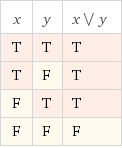
\includegraphics[scale=0.5]{eq_logic_or} \hspace{3pt}
                    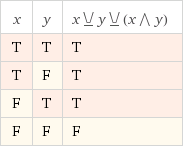
\includegraphics[scale=0.5]{eq_logic_or_anf}
                \end{figure}
            \end{block}

            \begin{block}{\normalsizeФункція NOT}
                \Large
                \begin{equation}
                    \nonumber
                    \neg x = x \oplus 1 \enspace.
                \end{equation}
            \end{block}
        \end{column}
    \end{columns}
\end{frame}


\begin{frame}{Побудова системи алгебраїчних рівнянь}{Опис бітових перестановок}
    \begin{columns}
        \begin{column}{0.48\textwidth}
            \begin{block}{}
                \begin{equation}
                    \nonumber
                    \left\{
                    \begin{array}{ll}
                        y_0 \oplus x_3 = 0; \\
                        y_1 \oplus x_2 = 0; \\
                        y_2 \oplus x_0 = 0; \\
                        y_3 \oplus x_1 = 0. \\
                    \end{array} \right.
                \end{equation}
            \end{block}
            \begin{block}{}
                \begin{itemize}
                    \item 4 рівняння від 8 змінних;
                    \item бітовий зсув описується аналогічно;
                    \item за можливості варто уникати додавання нових рівнянь
                        та реалізовувати перестановку безпосередньою зміною
                        порядку невідомих.
                \end{itemize}
            \end{block}
        \end{column}%
        \begin{column}{0.5\textwidth}
            \hspace{1em}
            \begin{block}{Бітова перестановка}
                \begin{figure}[htbp]
                    \centering
                    \vspace{6ex}
                    % Graphic for TeX using PGF
% Title: /home/zoresvit/devel/texmf/dstu-3008-95/images/eq_permutation.dia
% Creator: Dia v0.97.2
% CreationDate: Mon Jun  3 02:38:01 2013
% For: zoresvit
% \usepackage{tikz}
% The following commands are not supported in PSTricks at present
% We define them conditionally, so when they are implemented,
% this pgf file will use them.
\ifx\du\undefined
  \newlength{\du}
\fi
\setlength{\du}{15\unitlength}
\begin{tikzpicture}
\pgftransformxscale{1.000000}
\pgftransformyscale{-1.000000}
\definecolor{dialinecolor}{rgb}{0.000000, 0.000000, 0.000000}
\pgfsetstrokecolor{dialinecolor}
\definecolor{dialinecolor}{rgb}{1.000000, 1.000000, 1.000000}
\pgfsetfillcolor{dialinecolor}
\pgfsetlinewidth{0.100000\du}
\pgfsetdash{}{0pt}
\pgfsetdash{}{0pt}
\pgfsetbuttcap
{
\definecolor{dialinecolor}{rgb}{0.000000, 0.000000, 0.000000}
\pgfsetfillcolor{dialinecolor}
% was here!!!
\definecolor{dialinecolor}{rgb}{0.000000, 0.000000, 0.000000}
\pgfsetstrokecolor{dialinecolor}
\draw (19.000000\du,5.000000\du)--(19.000000\du,6.000000\du);
}
\pgfsetlinewidth{0.100000\du}
\pgfsetdash{}{0pt}
\pgfsetdash{}{0pt}
\pgfsetbuttcap
{
\definecolor{dialinecolor}{rgb}{0.000000, 0.000000, 0.000000}
\pgfsetfillcolor{dialinecolor}
% was here!!!
\definecolor{dialinecolor}{rgb}{0.000000, 0.000000, 0.000000}
\pgfsetstrokecolor{dialinecolor}
\draw (24.000000\du,5.000000\du)--(24.000000\du,6.000000\du);
}
\pgfsetlinewidth{0.100000\du}
\pgfsetdash{}{0pt}
\pgfsetdash{}{0pt}
\pgfsetbuttcap
{
\definecolor{dialinecolor}{rgb}{0.000000, 0.000000, 0.000000}
\pgfsetfillcolor{dialinecolor}
% was here!!!
\definecolor{dialinecolor}{rgb}{0.000000, 0.000000, 0.000000}
\pgfsetstrokecolor{dialinecolor}
\draw (21.500000\du,5.000000\du)--(21.500000\du,6.000000\du);
}
\pgfsetlinewidth{0.100000\du}
\pgfsetdash{}{0pt}
\pgfsetdash{}{0pt}
\pgfsetbuttcap
{
\definecolor{dialinecolor}{rgb}{0.000000, 0.000000, 0.000000}
\pgfsetfillcolor{dialinecolor}
% was here!!!
\definecolor{dialinecolor}{rgb}{0.000000, 0.000000, 0.000000}
\pgfsetstrokecolor{dialinecolor}
\draw (26.500000\du,5.000000\du)--(26.500000\du,6.000000\du);
}
\pgfsetlinewidth{0.100000\du}
\pgfsetdash{}{0pt}
\pgfsetdash{}{0pt}
\pgfsetbuttcap
{
\definecolor{dialinecolor}{rgb}{0.000000, 0.000000, 0.000000}
\pgfsetfillcolor{dialinecolor}
% was here!!!
\definecolor{dialinecolor}{rgb}{0.000000, 0.000000, 0.000000}
\pgfsetstrokecolor{dialinecolor}
\draw (19.000000\du,10.000000\du)--(19.000000\du,11.000000\du);
}
\pgfsetlinewidth{0.100000\du}
\pgfsetdash{}{0pt}
\pgfsetdash{}{0pt}
\pgfsetbuttcap
{
\definecolor{dialinecolor}{rgb}{0.000000, 0.000000, 0.000000}
\pgfsetfillcolor{dialinecolor}
% was here!!!
\definecolor{dialinecolor}{rgb}{0.000000, 0.000000, 0.000000}
\pgfsetstrokecolor{dialinecolor}
\draw (24.000000\du,10.000000\du)--(24.000000\du,11.000000\du);
}
\pgfsetlinewidth{0.100000\du}
\pgfsetdash{}{0pt}
\pgfsetdash{}{0pt}
\pgfsetbuttcap
{
\definecolor{dialinecolor}{rgb}{0.000000, 0.000000, 0.000000}
\pgfsetfillcolor{dialinecolor}
% was here!!!
\definecolor{dialinecolor}{rgb}{0.000000, 0.000000, 0.000000}
\pgfsetstrokecolor{dialinecolor}
\draw (21.500000\du,10.000000\du)--(21.500000\du,11.000000\du);
}
\pgfsetlinewidth{0.100000\du}
\pgfsetdash{}{0pt}
\pgfsetdash{}{0pt}
\pgfsetbuttcap
{
\definecolor{dialinecolor}{rgb}{0.000000, 0.000000, 0.000000}
\pgfsetfillcolor{dialinecolor}
% was here!!!
\definecolor{dialinecolor}{rgb}{0.000000, 0.000000, 0.000000}
\pgfsetstrokecolor{dialinecolor}
\draw (26.500000\du,10.000000\du)--(26.500000\du,11.000000\du);
}
\pgfsetlinewidth{0.100000\du}
\pgfsetdash{}{0pt}
\pgfsetdash{}{0pt}
\pgfsetbuttcap
{
\definecolor{dialinecolor}{rgb}{0.000000, 0.000000, 0.000000}
\pgfsetfillcolor{dialinecolor}
% was here!!!
\definecolor{dialinecolor}{rgb}{0.000000, 0.000000, 0.000000}
\pgfsetstrokecolor{dialinecolor}
\draw (19.000000\du,6.000000\du)--(26.500000\du,10.000000\du);
}
\pgfsetlinewidth{0.100000\du}
\pgfsetdash{}{0pt}
\pgfsetdash{}{0pt}
\pgfsetbuttcap
{
\definecolor{dialinecolor}{rgb}{0.000000, 0.000000, 0.000000}
\pgfsetfillcolor{dialinecolor}
% was here!!!
\definecolor{dialinecolor}{rgb}{0.000000, 0.000000, 0.000000}
\pgfsetstrokecolor{dialinecolor}
\draw (21.500000\du,6.000000\du)--(24.000000\du,10.000000\du);
}
\pgfsetlinewidth{0.100000\du}
\pgfsetdash{}{0pt}
\pgfsetdash{}{0pt}
\pgfsetbuttcap
{
\definecolor{dialinecolor}{rgb}{0.000000, 0.000000, 0.000000}
\pgfsetfillcolor{dialinecolor}
% was here!!!
\definecolor{dialinecolor}{rgb}{0.000000, 0.000000, 0.000000}
\pgfsetstrokecolor{dialinecolor}
\draw (24.000000\du,6.000000\du)--(21.500000\du,10.000000\du);
}
\pgfsetlinewidth{0.100000\du}
\pgfsetdash{}{0pt}
\pgfsetdash{}{0pt}
\pgfsetbuttcap
{
\definecolor{dialinecolor}{rgb}{0.000000, 0.000000, 0.000000}
\pgfsetfillcolor{dialinecolor}
% was here!!!
\definecolor{dialinecolor}{rgb}{0.000000, 0.000000, 0.000000}
\pgfsetstrokecolor{dialinecolor}
\draw (26.500000\du,6.000000\du)--(19.000000\du,10.000000\du);
}
% setfont left to latex
\definecolor{dialinecolor}{rgb}{0.000000, 0.000000, 0.000000}
\pgfsetstrokecolor{dialinecolor}
\node[anchor=west] at (18.000000\du,4.500000\du){$x_0$};
% setfont left to latex
\definecolor{dialinecolor}{rgb}{0.000000, 0.000000, 0.000000}
\pgfsetstrokecolor{dialinecolor}
\node[anchor=west] at (20.500000\du,4.500000\du){$x_1$};
% setfont left to latex
\definecolor{dialinecolor}{rgb}{0.000000, 0.000000, 0.000000}
\pgfsetstrokecolor{dialinecolor}
\node[anchor=west] at (23.000000\du,4.500000\du){$x_2$};
% setfont left to latex
\definecolor{dialinecolor}{rgb}{0.000000, 0.000000, 0.000000}
\pgfsetstrokecolor{dialinecolor}
\node[anchor=west] at (26.000000\du,4.500000\du){$x_3$};
% setfont left to latex
\definecolor{dialinecolor}{rgb}{0.000000, 0.000000, 0.000000}
\pgfsetstrokecolor{dialinecolor}
\node[anchor=west] at (18.000000\du,12.000000\du){$y_0$};
% setfont left to latex
\definecolor{dialinecolor}{rgb}{0.000000, 0.000000, 0.000000}
\pgfsetstrokecolor{dialinecolor}
\node[anchor=west] at (20.500000\du,12.000000\du){$y_1$};
% setfont left to latex
\definecolor{dialinecolor}{rgb}{0.000000, 0.000000, 0.000000}
\pgfsetstrokecolor{dialinecolor}
\node[anchor=west] at (23.000000\du,12.000000\du){$y_2$};
% setfont left to latex
\definecolor{dialinecolor}{rgb}{0.000000, 0.000000, 0.000000}
\pgfsetstrokecolor{dialinecolor}
\node[anchor=west] at (26.000000\du,12.000000\du){$y_3$};
\end{tikzpicture}

                    \vspace{6ex}
                \end{figure}
            \end{block}
        \end{column}
    \end{columns}
\end{frame}

\begin{frame}{Побудова системи алгебраїчних рівнянь}{Опис модульного додавання}
    \begin{block}{Стандартний опис модульного додавання}
        \begin{itemize}
                \small
            \item $R = X + Y \mod n \enspace;$ \\
                $ X = (x_0, \hdots, x_{n-1}) \enspace; \; 
                Y = (y_0, \hdots, y_{n-1}) \enspace; \;
                R = (r_0, \hdots, r_{n-1}) \enspace; $
            \item 
                $r_i = x_i \oplus y_i \oplus c_{i-1} \enspace;$ \hspace{4ex} 
                $c_i = r_{i+1} \oplus x_{i+1} \oplus y_{i+1} \enspace.$
        \end{itemize}
    \end{block}
    \begin{block}{}
        \begin{itemize}
                \small
            \item Головна мета --- описати суматор системой рівнянь другого степеня,
                не вводячи додаткових змінних для бітів переносу.
            \item $0 < i < (n - 1)$: \\
                $(x_i \oplus r_i) (x_i \oplus c_i) = 0 \enspace;$ \\
                $(y_i \oplus r_i) (y_i \oplus c_i) = 0 \enspace;$ \\
                $(x_i \oplus y_i) \cdot r_i \oplus x_i y_i \oplus x_i \oplus y_i \oplus c_i = 0 \enspace.$
        \end{itemize}
    \end{block}
    \begin{block}{Опис суматора рівняннями другого степеня}
        \small
        $\color{blue} r_0 = x_0 \oplus y_0 \enspace;$ \\
        $x_i \oplus x_i r_i \oplus x_i r_{i+1} \oplus x_i x_{i+1} \oplus x_i y_{i+1} \oplus r_i r_{i+1} \oplus r_i x_{i+1} \oplus r_i y_{i+1} = 0 \enspace;$ \\
        $y_i \oplus y_i r_i \oplus y_i r_{i+1} \oplus y_i x_{i+1} \oplus y_i y_{i+1} \oplus r_i r_{i+1} \oplus r_i x_{i+1} \oplus r_i y_{i+1} = 0 \enspace;$ \\
        $x_i r_i \oplus y_i r_i \oplus x_i y_i \oplus x_i \oplus y_i \oplus r_{i+1} \oplus x_{i+1} \oplus y_{i+1} = 0 \enspace.$ 
    \end{block}
\end{frame}

\begin{frame}{Побудова системи алгебраїчних рівнянь}{Опис S-блоків}
    \begin{columns}
        \begin{column}{0.5\textwidth}
            \begin{block}{Підстановка 8-го степеня}
                \begin{equation}
                    \nonumber
                    \left(
                    \begin{array}{ll}
                        0\; 1\; 2\; 3\; 4\; 5\; 6\; 7 \\
                        7\; 6\; 0\; 4\; 2\; 5\; 1\; 3 
                    \end{array} \right)
                \end{equation}
            \end{block}
            \begin{block}{}
                \begin{enumerate}
                    \item Побудова матриці $8 \times 22$; \\
                        {\small
                        кожний рядок містить значення кожного з $22$ мономів
                        для кожного з $8$ можливих вхідних значень;}
                    \item пошук ядра лінійного відображення \\
                        {\small(вирішення методом Гауса);} 
                    \item підстановка описується 14 рівняннями.
                \end{enumerate}
            \end{block}

        \end{column}%

        \begin{column}{0.5\textwidth}
            \small
            \begin{equation}
                \nonumber
                \left(
                \begin{array}{lllllllll}
                    1 & 1 & 1 & 1 & 1 & 1 & 1 & 1 & 1       \\[-0.5ex]
                    0 & 0 & 0 & 0 & 1 & 1 & 1 & 1 & x_0     \\[-0.5ex]
                    0 & 0 & 1 & 1 & 0 & 0 & 1 & 1 & x_1     \\[-0.5ex]
                    0 & 1 & 0 & 1 & 0 & 1 & 0 & 1 & x_2     \\[-0.5ex]
                    1 & 1 & 0 & 1 & 0 & 1 & 0 & 0 & y_0     \\[-0.5ex]
                    1 & 1 & 0 & 0 & 1 & 0 & 0 & 1 & y_1     \\[-0.5ex]
                    1 & 0 & 0 & 0 & 0 & 1 & 1 & 1 & y_2     \\[-0.5ex]
                    0 & 0 & 0 & 0 & 0 & 0 & 1 & 1 & x_0 x_1 \\[-0.5ex]
                    0 & 0 & 0 & 0 & 0 & 1 & 0 & 1 & x_0 x_2 \\[-0.5ex]
                    0 & 0 & 0 & 0 & 0 & 1 & 0 & 0 & x_0 y_0 \\[-0.5ex]
                    0 & 0 & 0 & 0 & 1 & 0 & 0 & 1 & x_0 y_1 \\[-0.5ex]
                    0 & 0 & 0 & 0 & 0 & 1 & 1 & 1 & x_0 y_2 \\[-0.5ex]
                    0 & 0 & 0 & 1 & 0 & 0 & 0 & 1 & x_1 x_2 \\[-0.5ex]
                    0 & 0 & 0 & 1 & 0 & 0 & 0 & 0 & x_1 y_0 \\[-0.5ex]
                    0 & 0 & 0 & 0 & 0 & 0 & 0 & 1 & x_1 y_1 \\[-0.5ex]
                    0 & 0 & 0 & 0 & 0 & 0 & 1 & 1 & x_1 y_2 \\[-0.5ex]
                    0 & 1 & 0 & 1 & 0 & 1 & 0 & 0 & x_2 y_0 \\[-0.5ex]
                    0 & 1 & 0 & 0 & 0 & 0 & 0 & 1 & x_2 y_1 \\[-0.5ex]
                    0 & 0 & 0 & 0 & 0 & 1 & 0 & 1 & x_2 y_2 \\[-0.5ex]
                    1 & 1 & 0 & 0 & 0 & 0 & 0 & 0 & y_0 y_1 \\[-0.5ex]
                    1 & 0 & 0 & 0 & 0 & 1 & 0 & 0 & y_0 y_2 \\[-0.5ex]
                    1 & 0 & 0 & 0 & 0 & 0 & 0 & 1 & y_1 y_2
                \end{array} \right)
            \end{equation}
        \end{column}%
    \end{columns}
\end{frame}

\begin{frame}{Побудова системи алгебраїчних рівнянь}{Опис S-блоків}
    \small
    \begin{equation}
        \nonumber
        \left(
        \begin{array}{llllllllr}
            1 & 0 & 0 & 0 & 0 & 0 & 0 & 0 & x_0 y_0+ x_1+ x_2+ y_0+ y_1+ 1              \\[-0.5ex]
            0 & 1 & 0 & 0 & 0 & 0 & 0 & 0 & x_0 y_0+ x_0+ x_1+ y_2+ 1                   \\[-0.5ex] 
            0 & 0 & 1 & 0 & 0 & 0 & 0 & 0 & x_0 y_0+ x_0+ y_0+ 1                        \\[-0.5ex] 
            0 & 0 & 0 & 1 & 0 & 0 & 0 & 0 & x_0 y_0+ x_0+ x_2+ y_1+ y_2                 \\[-0.5ex] 
            0 & 0 & 0 & 0 & 1 & 0 & 0 & 0 & x_0 y_0+ x_0+ x_1+ x_2+ y_0+ y_1+ y_2+ 1    \\[-0.5ex] 
            0 & 0 & 0 & 0 & 0 & 1 & 0 & 0 & x_0 y_0                                     \\[-0.5ex] 
            0 & 0 & 0 & 0 & 0 & 0 & 1 & 0 & x_0 y_0+ x_2+ y_0+ y_2                      \\[-0.5ex] 
            0 & 0 & 0 & 0 & 0 & 0 & 0 & 1 & x_0 y_0+ x_1+ y_1+ 1                        \\[-0.5ex] 
            0 & 0 & 0 & 0 & 0 & 0 & 0 & 0 & \color{blue}x_0 x_2+ x_1+ y_1+ 1                        \\[-0.5ex] 
            0 & 0 & 0 & 0 & 0 & 0 & 0 & 0 & \color{blue}x_0 x_1+ x_1+ x_2+ y_0+ y_1+ y_2+ 1         \\[-0.5ex] 
            0 & 0 & 0 & 0 & 0 & 0 & 0 & 0 & \color{blue}x_0 y_1+ x_0+ x_2+ y_0+ y_2                 \\[-0.5ex] 
            0 & 0 & 0 & 0 & 0 & 0 & 0 & 0 & \color{blue}x_0 y_0+ x_0y_2+ x_1+ x_2+ y_0+ y_1+ y_2+ 1 \\[-0.5ex] 
            0 & 0 & 0 & 0 & 0 & 0 & 0 & 0 & \color{blue}x_1 x_2+ x_0+ x_1+ x_2+ y_2+ 1              \\[-0.5ex] 
            0 & 0 & 0 & 0 & 0 & 0 & 0 & 0 & \color{blue}x_0 y_0+ x_1y_0+ x_0+ x_2+ y_1+ y_2         \\[-0.5ex] 
            0 & 0 & 0 & 0 & 0 & 0 & 0 & 0 & \color{blue}x_0 y_0+ x_1y_1+ x_1+ y_1+ 1                \\[-0.5ex] 
            0 & 0 & 0 & 0 & 0 & 0 & 0 & 0 & \color{blue}x_1 y_2+ x_1+ x_2+ y_0+ y_1+ y_2+ 1         \\[-0.5ex] 
            0 & 0 & 0 & 0 & 0 & 0 & 0 & 0 & \color{blue}x_0 y_0+ x_2y_0+ x_1+ x_2+ y_1+ 1           \\[-0.5ex] 
            0 & 0 & 0 & 0 & 0 & 0 & 0 & 0 & \color{blue}x_2 y_1+ x_0+ y_1+ y_2                      \\[-0.5ex] 
            0 & 0 & 0 & 0 & 0 & 0 & 0 & 0 & \color{blue}x_2 y_2+ x_1+ y_1+ 1                        \\[-0.5ex] 
            0 & 0 & 0 & 0 & 0 & 0 & 0 & 0 & \color{blue}y_0 y_1+ x_0+ x_2+ y_0+ y_1+ y_2            \\[-0.5ex] 
            0 & 0 & 0 & 0 & 0 & 0 & 0 & 0 & \color{blue}y_0 y_2+ x_1+ x_2+ y_0+ y_1+ 1              \\[-0.5ex] 
            0 & 0 & 0 & 0 & 0 & 0 & 0 & 0 & \color{blue}y_1 y_2+ x_2+ y_0                            
        \end{array} \right)
    \end{equation} 
\end{frame}

\begin{frame}[shrink]{Методи вирішення систем нелінійних рівнянь}
    \begin{block}{Зведений базис Ґробнера}
        \begin{itemize}
            \item узагальнення методу Гауса для систем нелінійних рівнянь;
            \item алгоритми Бухберґера, $F4$, $F5$.
        \end{itemize}
    \end{block}
    \begin{exampleblock}{Задача здійснимості бульових формул (SAT-solvers)}
        \begin{itemize}
            \item пошук значень змінних, що задовольняють систему рівнянь.
        \end{itemize}        
    \end{exampleblock}
    \begin{block}{Цілочислове лінійне програмування (Mixed Integer Solvers)}
        \begin{itemize}
            \item вирішення екстремальної задачі --- знаходження мінімуму  \\
                (або максимуму) функції при заданих обмеженнях.
        \end{itemize}
    \end{block}

    \begin{block}{Алгебраїчні диференціали вищого порядку}
    \begin{itemize}
        \item ``кубічні атаки'' --- представлення функції шифрування у виді
            поліноміальних рівнянь низького степеня
    \end{itemize}
    \end{block}
\end{frame}

\begin{frame}[shrink]{Блоковий симетричний шифр ГОСТ~28147-89}{Система алгебраїчних рівнянь}
    \begin{columns}
        \begin{column}{0.52\textwidth}
            \begin{block}{Змінні одного раунда}
                \begin{description}
                    \item[$X_{r, \, 0 \hdots 63}$]  вхідний блок;
                    \item[$K_{r \% 8, \, 0 \hdots 31}$]  біти ключа;
                    \item[$Y_{r, \, 0 \hdots 31}$]  результат додавання;
                    \item[$Z_{r, \, 0 \hdots 31}$]  результат заміни;
                    \item[$X_{r+1, \, 0 \hdots 63}$]  вихід раунда.
                \end{description}
            \end{block}
        \end{column}
        \begin{column}{0.5\textwidth}
            \begin{figure}[htbp]
                \centering
                % Graphic for TeX using PGF
% Title: /home/zoresvit/Documents/diploma/bachelor-thesis/images/gost.dia
% Creator: Dia v0.97.1
% CreationDate: Wed May  9 22:47:17 2012
% For: zoresvit
% \usepackage{tikz}
% The following commands are not supported in PSTricks at present
% We define them conditionally, so when they are implemented,
% this pgf file will use them.
\ifx\du\undefined
  \newlength{\du}
\fi
\setlength{\du}{15\unitlength}
\begin{tikzpicture}[every node/.style={scale=0.8}]
\pgftransformxscale{1.000000}
\pgftransformyscale{-1.000000}
\definecolor{dialinecolor}{rgb}{0.000000, 0.000000, 0.000000}
\pgfsetstrokecolor{dialinecolor}
\definecolor{dialinecolor}{rgb}{1.000000, 1.000000, 1.000000}
\pgfsetfillcolor{dialinecolor}
\definecolor{dialinecolor}{rgb}{1.000000, 1.000000, 1.000000}
\pgfsetfillcolor{dialinecolor}
\fill (16.000000\du,2.000000\du)--(16.000000\du,4.000000\du)--(28.000000\du,4.000000\du)--(28.000000\du,2.000000\du)--cycle;
\pgfsetlinewidth{0.100000\du}
\pgfsetdash{}{0pt}
\pgfsetdash{}{0pt}
\pgfsetmiterjoin
\definecolor{dialinecolor}{rgb}{0.000000, 0.000000, 0.000000}
\pgfsetstrokecolor{dialinecolor}
\draw (16.000000\du,2.000000\du)--(16.000000\du,4.000000\du)--(28.000000\du,4.000000\du)--(28.000000\du,2.000000\du)--cycle;
% setfont left to latex
\definecolor{dialinecolor}{rgb}{0.000000, 0.000000, 0.000000}
\pgfsetstrokecolor{dialinecolor}
\node at (22.000000\du,3.000000\du){INPUT};
\definecolor{dialinecolor}{rgb}{1.000000, 1.000000, 1.000000}
\pgfsetfillcolor{dialinecolor}
\fill (16.000000\du,12.000000\du)--(16.000000\du,14.000000\du)--(28.000000\du,14.000000\du)--(28.000000\du,12.000000\du)--cycle;
\pgfsetlinewidth{0.100000\du}
\pgfsetdash{}{0pt}
\pgfsetdash{}{0pt}
\pgfsetmiterjoin
\definecolor{dialinecolor}{rgb}{0.000000, 0.000000, 0.000000}
\pgfsetstrokecolor{dialinecolor}
\draw (16.000000\du,12.000000\du)--(16.000000\du,14.000000\du)--(28.000000\du,14.000000\du)--(28.000000\du,12.000000\du)--cycle;
% setfont left to latex
\definecolor{dialinecolor}{rgb}{0.000000, 0.000000, 0.000000}
\pgfsetstrokecolor{dialinecolor}
\node at (22.000000\du,13.000000\du){OUTPUT};
\definecolor{dialinecolor}{rgb}{1.000000, 1.000000, 1.000000}
\pgfsetfillcolor{dialinecolor}
\fill (30.000000\du,2.000000\du)--(30.000000\du,4.000000\du)--(36.000000\du,4.000000\du)--(36.000000\du,2.000000\du)--cycle;
\pgfsetlinewidth{0.100000\du}
\pgfsetdash{}{0pt}
\pgfsetdash{}{0pt}
\pgfsetmiterjoin
\definecolor{dialinecolor}{rgb}{0.000000, 0.000000, 0.000000}
\pgfsetstrokecolor{dialinecolor}
\draw (30.000000\du,2.000000\du)--(30.000000\du,4.000000\du)--(36.000000\du,4.000000\du)--(36.000000\du,2.000000\du)--cycle;
% setfont left to latex
\definecolor{dialinecolor}{rgb}{0.000000, 0.000000, 0.000000}
\pgfsetstrokecolor{dialinecolor}
\node at (33.000000\du,3.000000\du){SUBKEY};
\pgfsetlinewidth{0.100000\du}
\pgfsetdash{}{0pt}
\pgfsetdash{}{0pt}
\pgfsetbuttcap
{
\definecolor{dialinecolor}{rgb}{0.000000, 0.000000, 0.000000}
\pgfsetfillcolor{dialinecolor}
% was here!!!
\definecolor{dialinecolor}{rgb}{0.000000, 0.000000, 0.000000}
\pgfsetstrokecolor{dialinecolor}
\draw (26.500000\du,4.500000\du)--(26.500000\du,8.000000\du);
}
\pgfsetlinewidth{0.100000\du}
\pgfsetdash{}{0pt}
\pgfsetdash{}{0pt}
\pgfsetmiterjoin
\pgfsetbuttcap
{
\definecolor{dialinecolor}{rgb}{0.000000, 0.000000, 0.000000}
\pgfsetfillcolor{dialinecolor}
% was here!!!
{\pgfsetcornersarced{\pgfpoint{0.000000\du}{0.000000\du}}\definecolor{dialinecolor}{rgb}{0.000000, 0.000000, 0.000000}
\pgfsetstrokecolor{dialinecolor}
\draw (33.000000\du,4.000000\du)--(33.000000\du,5.500000\du)--(26.754900\du,5.500000\du)--(26.754900\du,5.500000\du);
}}
\pgfsetlinewidth{0.100000\du}
\pgfsetdash{}{0pt}
\pgfsetdash{}{0pt}
\pgfsetmiterjoin
\definecolor{dialinecolor}{rgb}{1.000000, 1.000000, 1.000000}
\pgfsetfillcolor{dialinecolor}
\fill (24.800000\du,6.500000\du)--(24.800000\du,7.500000\du)--(25.800000\du,7.500000\du)--(25.800000\du,6.500000\du)--cycle;
\definecolor{dialinecolor}{rgb}{0.000000, 0.000000, 0.000000}
\pgfsetstrokecolor{dialinecolor}
\draw (24.800000\du,6.500000\du)--(24.800000\du,7.500000\du)--(25.800000\du,7.500000\du)--(25.800000\du,6.500000\du)--cycle;
\pgfsetlinewidth{0.100000\du}
\pgfsetdash{}{0pt}
\pgfsetdash{}{0pt}
\pgfsetbuttcap
{
\definecolor{dialinecolor}{rgb}{0.000000, 0.000000, 0.000000}
\pgfsetfillcolor{dialinecolor}
% was here!!!
\definecolor{dialinecolor}{rgb}{0.000000, 0.000000, 0.000000}
\pgfsetstrokecolor{dialinecolor}
\draw (25.300000\du,6.500000\du)--(25.300000\du,7.500000\du);
}
\pgfsetlinewidth{0.100000\du}
\pgfsetdash{}{0pt}
\pgfsetdash{}{0pt}
\pgfsetbuttcap
{
\definecolor{dialinecolor}{rgb}{0.000000, 0.000000, 0.000000}
\pgfsetfillcolor{dialinecolor}
% was here!!!
\definecolor{dialinecolor}{rgb}{0.000000, 0.000000, 0.000000}
\pgfsetstrokecolor{dialinecolor}
\draw (24.800000\du,7.000000\du)--(25.800000\du,7.000000\du);
}
% setfont left to latex
\definecolor{dialinecolor}{rgb}{0.000000, 0.000000, 0.000000}
\pgfsetstrokecolor{dialinecolor}
\node[anchor=west] at (27.200000\du,1.500000\du){0};
% setfont left to latex
\definecolor{dialinecolor}{rgb}{0.000000, 0.000000, 0.000000}
\pgfsetstrokecolor{dialinecolor}
\node[anchor=west] at (20.500000\du,1.500000\du){32 31};
% setfont left to latex
\definecolor{dialinecolor}{rgb}{0.000000, 0.000000, 0.000000}
\pgfsetstrokecolor{dialinecolor}
\node[anchor=west] at (15.500000\du,1.500000\du){63};
% setfont left to latex
\definecolor{dialinecolor}{rgb}{0.000000, 0.000000, 0.000000}
\pgfsetstrokecolor{dialinecolor}
\node[anchor=west] at (35.200000\du,1.500000\du){0};
% setfont left to latex
\definecolor{dialinecolor}{rgb}{0.000000, 0.000000, 0.000000}
\pgfsetstrokecolor{dialinecolor}
\node[anchor=west] at (29.500000\du,1.500000\du){31};
\pgfsetlinewidth{0.100000\du}
\pgfsetdash{}{0pt}
\pgfsetdash{}{0pt}
\pgfsetbuttcap
{
\definecolor{dialinecolor}{rgb}{0.000000, 0.000000, 0.000000}
\pgfsetfillcolor{dialinecolor}
% was here!!!
\definecolor{dialinecolor}{rgb}{0.000000, 0.000000, 0.000000}
\pgfsetstrokecolor{dialinecolor}
\pgfpathmoveto{\pgfpoint{26.800000\du}{5.546870\du}}
\pgfpatharc{360}{181}{0.300000\du and 0.300000\du}
\pgfusepath{stroke}
}
% setfont left to latex
\definecolor{dialinecolor}{rgb}{0.000000, 0.000000, 0.000000}
\pgfsetstrokecolor{dialinecolor}
\node[anchor=west] at (33.500000\du,5.000000\du){$K_i$};
\pgfsetlinewidth{0.100000\du}
\pgfsetdash{}{0pt}
\pgfsetdash{}{0pt}
\pgfsetbuttcap
{
\definecolor{dialinecolor}{rgb}{0.000000, 0.000000, 0.000000}
\pgfsetfillcolor{dialinecolor}
% was here!!!
\definecolor{dialinecolor}{rgb}{0.000000, 0.000000, 0.000000}
\pgfsetstrokecolor{dialinecolor}
\draw (26.500000\du,8.000000\du)--(17.500000\du,9.500000\du);
}
\pgfsetlinewidth{0.100000\du}
\pgfsetdash{}{0pt}
\pgfsetdash{}{0pt}
\pgfsetmiterjoin
\pgfsetbuttcap
{
\definecolor{dialinecolor}{rgb}{0.000000, 0.000000, 0.000000}
\pgfsetfillcolor{dialinecolor}
% was here!!!
\definecolor{dialinecolor}{rgb}{0.000000, 0.000000, 0.000000}
\pgfsetstrokecolor{dialinecolor}
\pgfpathmoveto{\pgfpoint{26.500000\du}{4.500000\du}}
\pgfpathcurveto{\pgfpoint{26.500000\du}{3.900000\du}}{\pgfpoint{22.000000\du}{4.600000\du}}{\pgfpoint{22.000000\du}{4.000000\du}}
\pgfusepath{stroke}
}
\pgfsetlinewidth{0.100000\du}
\pgfsetdash{}{0pt}
\pgfsetdash{}{0pt}
\pgfsetmiterjoin
\pgfsetbuttcap
{
\definecolor{dialinecolor}{rgb}{0.000000, 0.000000, 0.000000}
\pgfsetfillcolor{dialinecolor}
% was here!!!
\definecolor{dialinecolor}{rgb}{0.000000, 0.000000, 0.000000}
\pgfsetstrokecolor{dialinecolor}
\pgfpathmoveto{\pgfpoint{26.500000\du}{4.500000\du}}
\pgfpathcurveto{\pgfpoint{26.500000\du}{4.100000\du}}{\pgfpoint{28.000000\du}{4.600000\du}}{\pgfpoint{28.000000\du}{4.000000\du}}
\pgfusepath{stroke}
}
\pgfsetlinewidth{0.100000\du}
\pgfsetdash{}{0pt}
\pgfsetdash{}{0pt}
\pgfsetmiterjoin
\pgfsetbuttcap
{
\definecolor{dialinecolor}{rgb}{0.000000, 0.000000, 0.000000}
\pgfsetfillcolor{dialinecolor}
% was here!!!
\definecolor{dialinecolor}{rgb}{0.000000, 0.000000, 0.000000}
\pgfsetstrokecolor{dialinecolor}
\pgfpathmoveto{\pgfpoint{17.500000\du}{11.500000\du}}
\pgfpathcurveto{\pgfpoint{17.500000\du}{11.880000\du}}{\pgfpoint{16.000000\du}{11.500000\du}}{\pgfpoint{16.000000\du}{12.000000\du}}
\pgfusepath{stroke}
}
\pgfsetlinewidth{0.100000\du}
\pgfsetdash{}{0pt}
\pgfsetdash{}{0pt}
\pgfsetmiterjoin
\pgfsetbuttcap
{
\definecolor{dialinecolor}{rgb}{0.000000, 0.000000, 0.000000}
\pgfsetfillcolor{dialinecolor}
% was here!!!
\definecolor{dialinecolor}{rgb}{0.000000, 0.000000, 0.000000}
\pgfsetstrokecolor{dialinecolor}
\pgfpathmoveto{\pgfpoint{17.500000\du}{11.500000\du}}
\pgfpathcurveto{\pgfpoint{17.500000\du}{12.100000\du}}{\pgfpoint{22.000000\du}{11.300000\du}}{\pgfpoint{22.000000\du}{12.000000\du}}
\pgfusepath{stroke}
}
\pgfsetlinewidth{0.100000\du}
\pgfsetdash{}{0pt}
\pgfsetdash{}{0pt}
\pgfsetbuttcap
{
\definecolor{dialinecolor}{rgb}{0.000000, 0.000000, 0.000000}
\pgfsetfillcolor{dialinecolor}
% was here!!!
\pgfsetarrowsend{stealth}
\definecolor{dialinecolor}{rgb}{0.000000, 0.000000, 0.000000}
\pgfsetstrokecolor{dialinecolor}
\draw (17.500000\du,9.500000\du)--(17.500000\du,11.500000\du);
}
\definecolor{dialinecolor}{rgb}{1.000000, 1.000000, 1.000000}
\pgfsetfillcolor{dialinecolor}
\fill (21.700000\du,6.175000\du)--(21.700000\du,7.804167\du)--(23.982500\du,7.804167\du)--(23.982500\du,6.175000\du)--cycle;
\pgfsetlinewidth{0.100000\du}
\pgfsetdash{}{0pt}
\pgfsetdash{}{0pt}
\pgfsetmiterjoin
\definecolor{dialinecolor}{rgb}{0.000000, 0.000000, 0.000000}
\pgfsetstrokecolor{dialinecolor}
\draw (21.700000\du,6.175000\du)--(21.700000\du,7.804167\du)--(23.982500\du,7.804167\du)--(23.982500\du,6.175000\du)--cycle;
% setfont left to latex
\definecolor{dialinecolor}{rgb}{0.000000, 0.000000, 0.000000}
\pgfsetstrokecolor{dialinecolor}
\node at (22.841250\du,7.120000\du){S-box};
\pgfsetlinewidth{0.100000\du}
\pgfsetdash{}{0pt}
\pgfsetdash{}{0pt}
\pgfsetmiterjoin
\pgfsetbuttcap
{
\definecolor{dialinecolor}{rgb}{0.000000, 0.000000, 0.000000}
\pgfsetfillcolor{dialinecolor}
% was here!!!
\pgfsetarrowsend{stealth}
{\pgfsetcornersarced{\pgfpoint{0.000000\du}{0.000000\du}}\definecolor{dialinecolor}{rgb}{0.000000, 0.000000, 0.000000}
\pgfsetstrokecolor{dialinecolor}
\draw (26.247900\du,5.500000\du)--(26.247900\du,5.500000\du)--(25.300000\du,5.500000\du)--(25.300000\du,6.455078\du);
}}
\pgfsetlinewidth{0.100000\du}
\pgfsetdash{}{0pt}
\pgfsetdash{}{0pt}
\pgfsetbuttcap
{
\definecolor{dialinecolor}{rgb}{0.000000, 0.000000, 0.000000}
\pgfsetfillcolor{dialinecolor}
% was here!!!
\pgfsetarrowsend{stealth}
\definecolor{dialinecolor}{rgb}{0.000000, 0.000000, 0.000000}
\pgfsetstrokecolor{dialinecolor}
\draw (24.800000\du,7.000000\du)--(23.982500\du,6.989583\du);
}
\pgfsetlinewidth{0.100000\du}
\pgfsetdash{}{0pt}
\pgfsetdash{}{0pt}
\pgfsetmiterjoin
\pgfsetbuttcap
{
\definecolor{dialinecolor}{rgb}{0.000000, 0.000000, 0.000000}
\pgfsetfillcolor{dialinecolor}
% was here!!!
\definecolor{dialinecolor}{rgb}{0.000000, 0.000000, 0.000000}
\pgfsetstrokecolor{dialinecolor}
\pgfpathmoveto{\pgfpoint{17.500000\du}{4.500000\du}}
\pgfpathcurveto{\pgfpoint{17.500000\du}{4.100000\du}}{\pgfpoint{16.000000\du}{4.600000\du}}{\pgfpoint{16.000000\du}{4.000000\du}}
\pgfusepath{stroke}
}
\pgfsetlinewidth{0.100000\du}
\pgfsetdash{}{0pt}
\pgfsetdash{}{0pt}
\pgfsetmiterjoin
\pgfsetbuttcap
{
\definecolor{dialinecolor}{rgb}{0.000000, 0.000000, 0.000000}
\pgfsetfillcolor{dialinecolor}
% was here!!!
\definecolor{dialinecolor}{rgb}{0.000000, 0.000000, 0.000000}
\pgfsetstrokecolor{dialinecolor}
\pgfpathmoveto{\pgfpoint{17.500000\du}{4.500000\du}}
\pgfpathcurveto{\pgfpoint{17.500000\du}{4.000000\du}}{\pgfpoint{22.000000\du}{4.600000\du}}{\pgfpoint{22.000000\du}{4.000000\du}}
\pgfusepath{stroke}
}
\pgfsetlinewidth{0.100000\du}
\pgfsetdash{}{0pt}
\pgfsetdash{}{0pt}
\pgfsetmiterjoin
\definecolor{dialinecolor}{rgb}{1.000000, 1.000000, 1.000000}
\pgfsetfillcolor{dialinecolor}
\fill (18.800000\du,6.487500\du)--(18.800000\du,7.487500\du)--(20.800000\du,7.487500\du)--(20.800000\du,6.487500\du)--cycle;
\definecolor{dialinecolor}{rgb}{0.000000, 0.000000, 0.000000}
\pgfsetstrokecolor{dialinecolor}
\draw (18.800000\du,6.487500\du)--(18.800000\du,7.487500\du)--(20.800000\du,7.487500\du)--(20.800000\du,6.487500\du)--cycle;
% setfont left to latex
\definecolor{dialinecolor}{rgb}{0.000000, 0.000000, 0.000000}
\pgfsetstrokecolor{dialinecolor}
\node[anchor=west] at (18.600000\du,7.000000\du){$<<<$};
\pgfsetlinewidth{0.100000\du}
\pgfsetdash{}{0pt}
\pgfsetdash{}{0pt}
\pgfsetbuttcap
{
\definecolor{dialinecolor}{rgb}{0.000000, 0.000000, 0.000000}
\pgfsetfillcolor{dialinecolor}
% was here!!!
\pgfsetarrowsend{stealth}
\definecolor{dialinecolor}{rgb}{0.000000, 0.000000, 0.000000}
\pgfsetstrokecolor{dialinecolor}
\draw (21.700000\du,6.989583\du)--(20.800000\du,6.987500\du);
}
\pgfsetlinewidth{0.100000\du}
\pgfsetdash{}{0pt}
\pgfsetdash{}{0pt}
\pgfsetbuttcap
\pgfsetmiterjoin
\pgfsetlinewidth{0.100000\du}
\pgfsetbuttcap
\pgfsetmiterjoin
\pgfsetdash{}{0pt}
\definecolor{dialinecolor}{rgb}{1.000000, 1.000000, 1.000000}
\pgfsetfillcolor{dialinecolor}
\pgfpathellipse{\pgfpoint{17.500000\du}{7.000000\du}}{\pgfpoint{0.500000\du}{0\du}}{\pgfpoint{0\du}{0.500000\du}}
\pgfusepath{fill}
\definecolor{dialinecolor}{rgb}{0.000000, 0.000000, 0.000000}
\pgfsetstrokecolor{dialinecolor}
\pgfpathellipse{\pgfpoint{17.500000\du}{7.000000\du}}{\pgfpoint{0.500000\du}{0\du}}{\pgfpoint{0\du}{0.500000\du}}
\pgfusepath{stroke}
\pgfsetbuttcap
\pgfsetmiterjoin
\pgfsetdash{}{0pt}
\definecolor{dialinecolor}{rgb}{0.000000, 0.000000, 0.000000}
\pgfsetstrokecolor{dialinecolor}
\draw (17.500000\du,6.500000\du)--(17.500000\du,7.500000\du);
\pgfsetbuttcap
\pgfsetmiterjoin
\pgfsetdash{}{0pt}
\definecolor{dialinecolor}{rgb}{0.000000, 0.000000, 0.000000}
\pgfsetstrokecolor{dialinecolor}
\draw (17.000000\du,7.000000\du)--(18.000000\du,7.000000\du);
\pgfsetlinewidth{0.100000\du}
\pgfsetdash{}{0pt}
\pgfsetdash{}{0pt}
\pgfsetbuttcap
{
\definecolor{dialinecolor}{rgb}{0.000000, 0.000000, 0.000000}
\pgfsetfillcolor{dialinecolor}
% was here!!!
\pgfsetarrowsend{stealth}
\definecolor{dialinecolor}{rgb}{0.000000, 0.000000, 0.000000}
\pgfsetstrokecolor{dialinecolor}
\draw (18.800000\du,6.987500\du)--(18.000000\du,7.000000\du);
}
\pgfsetlinewidth{0.100000\du}
\pgfsetdash{}{0pt}
\pgfsetdash{}{0pt}
\pgfsetbuttcap
{
\definecolor{dialinecolor}{rgb}{0.000000, 0.000000, 0.000000}
\pgfsetfillcolor{dialinecolor}
% was here!!!
\definecolor{dialinecolor}{rgb}{0.000000, 0.000000, 0.000000}
\pgfsetstrokecolor{dialinecolor}
\draw (17.500000\du,4.500000\du)--(17.500000\du,6.500000\du);
}
\pgfsetlinewidth{0.100000\du}
\pgfsetdash{}{0pt}
\pgfsetdash{}{0pt}
\pgfsetbuttcap
{
\definecolor{dialinecolor}{rgb}{0.000000, 0.000000, 0.000000}
\pgfsetfillcolor{dialinecolor}
% was here!!!
\definecolor{dialinecolor}{rgb}{0.000000, 0.000000, 0.000000}
\pgfsetstrokecolor{dialinecolor}
\draw (17.500000\du,7.500000\du)--(17.500000\du,8.000000\du);
}
\pgfsetlinewidth{0.100000\du}
\pgfsetdash{}{0pt}
\pgfsetdash{}{0pt}
\pgfsetbuttcap
{
\definecolor{dialinecolor}{rgb}{0.000000, 0.000000, 0.000000}
\pgfsetfillcolor{dialinecolor}
% was here!!!
\definecolor{dialinecolor}{rgb}{0.000000, 0.000000, 0.000000}
\pgfsetstrokecolor{dialinecolor}
\draw (17.500000\du,8.000000\du)--(26.500000\du,9.500000\du);
}
\pgfsetlinewidth{0.100000\du}
\pgfsetdash{}{0pt}
\pgfsetdash{}{0pt}
\pgfsetmiterjoin
\pgfsetbuttcap
{
\definecolor{dialinecolor}{rgb}{0.000000, 0.000000, 0.000000}
\pgfsetfillcolor{dialinecolor}
% was here!!!
\definecolor{dialinecolor}{rgb}{0.000000, 0.000000, 0.000000}
\pgfsetstrokecolor{dialinecolor}
\pgfpathmoveto{\pgfpoint{26.500000\du}{11.500000\du}}
\pgfpathcurveto{\pgfpoint{26.500000\du}{12.000000\du}}{\pgfpoint{22.000000\du}{11.300000\du}}{\pgfpoint{22.000000\du}{12.000000\du}}
\pgfusepath{stroke}
}
\pgfsetlinewidth{0.100000\du}
\pgfsetdash{}{0pt}
\pgfsetdash{}{0pt}
\pgfsetmiterjoin
\pgfsetbuttcap
{
\definecolor{dialinecolor}{rgb}{0.000000, 0.000000, 0.000000}
\pgfsetfillcolor{dialinecolor}
% was here!!!
\definecolor{dialinecolor}{rgb}{0.000000, 0.000000, 0.000000}
\pgfsetstrokecolor{dialinecolor}
\pgfpathmoveto{\pgfpoint{26.500000\du}{11.500000\du}}
\pgfpathcurveto{\pgfpoint{26.500000\du}{11.900000\du}}{\pgfpoint{28.000000\du}{11.400000\du}}{\pgfpoint{28.000000\du}{12.000000\du}}
\pgfusepath{stroke}
}
\pgfsetlinewidth{0.100000\du}
\pgfsetdash{}{0pt}
\pgfsetdash{}{0pt}
\pgfsetbuttcap
{
\definecolor{dialinecolor}{rgb}{0.000000, 0.000000, 0.000000}
\pgfsetfillcolor{dialinecolor}
% was here!!!
\pgfsetarrowsend{stealth}
\definecolor{dialinecolor}{rgb}{0.000000, 0.000000, 0.000000}
\pgfsetstrokecolor{dialinecolor}
\draw (26.500000\du,9.500000\du)--(26.500000\du,11.500000\du);
}
\pgfsetlinewidth{0.100000\du}
\pgfsetdash{}{0pt}
\pgfsetdash{}{0pt}
\pgfsetbuttcap
{
\definecolor{dialinecolor}{rgb}{0.000000, 0.000000, 0.000000}
\pgfsetfillcolor{dialinecolor}
% was here!!!
\pgfsetarrowsend{stealth}
\definecolor{dialinecolor}{rgb}{0.000000, 0.000000, 0.000000}
\pgfsetstrokecolor{dialinecolor}
\draw (26.500000\du,7.000000\du)--(25.800000\du,7.000000\du);
}
\end{tikzpicture}

            \end{figure}
        \end{column}
    \end{columns}
    \begin{block}{Характеристика системи}
        \begin{itemize}
            \item $31 \cdot 3 + 1 = 94$ рівняння для складання з ключем;
            \item $21 \cdot 8 = 168$ рівнянь для S-блоків;
            \item один раунд шифру містить $325$ поліномів другого степеня;
            \item повний шифр --- $10432$ рівняння від $4416$ змінних \\
                (при використанні S-блоків з ГОСТ~34.311);
        \end{itemize}
    \end{block}
\end{frame}

\begin{frame}[shrink]{Блоковий симетричний шифр ГОСТ~28147-89}{Алгебраїчний криптоаналіз}
    \begin{block}{Апаратне забезпечення}
        \begin{description}
            \item[CPU] Intel Core i3;
            \item[RAM] 16~Gb RAM;
            \item[OS] Gentoo Linux ;
            \item[Software] Sage v5.6;\\
                CryptoMiniSat v2.8.
        \end{description}
    \end{block}
    \begin{block}{Атака}
        \begin{itemize}
            \item Використано 4 пари відкритого та шифрованого тексту;
            \item Відновлено 192 біти використаного підключа (6 раундів);
            \item Вирішено систему 1950 рівнянь від 828 змінних.
            \item Час обчислення $~40$ год.
        \end{itemize}
    \end{block}
\end{frame}

\begin{frame}{Блоковий симетричний шифр MISTY1}
    \begin{changemargin}{-2cm}{-2cm}
        \begin{figure}[htbp]
            \centering
            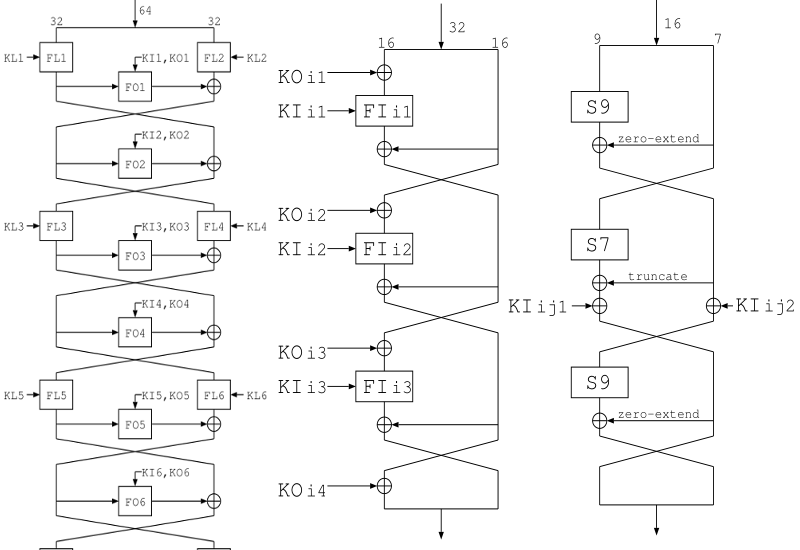
\includegraphics[scale=0.4]{misty}
        \end{figure}
    \end{changemargin}
\end{frame}

\begin{frame}{Блоковий симетричний шифр MISTY1}{S-блоки}
    \begin{changemargin}{-2cm}{-2cm}
        \small
        \begin{block}{S-блок $S_7$}
            \begin{equation}
                \nonumber
                \label{eqn:misty-s7}
                \begin{array}{ll}
                    y_0 =& x_0 + x_1 x_3 + x_0 x_3 x_4 + x_1 x_5 + x_0 x_2 x_5 + x_4 x_5 + \\
                    & + x_0 x_1 x_6 + x_2 x_6 + x_0 x_5 x_6 + x_3 x_5 x_6 + 1 \\
                    y_1 =& x_0 x_2 + x_0 x_4 +x_3 x_4 +x_1 x_5 + x_2 x_4 x_5 +x_6 + \\
                    & + x_0 x_6 +x_3 x_6 +x_2 x_3 x_6 + x_1 x_4 x_6 + x_0 x_5 x_6 +1 \\
                    y_2 =& x_1 x_2 + x_0 x_2 x_3 + x_4 + x_1 x_4 + x_0 x_1 x_4 + x_0 x_5 + x_0 x_4 x_5 + \\
                    & + x_3 x_4 x_5 + x_1 x_6 + x_3 x_6 + x_0 x_3 x_6 + x_4 x_6 + x_2 x_4 x_6 \\
                    y_3 =& x_0 + x_1 + x_0 x_1 x_2 + x_0 x_3 + x_2 x_4 + x_1 x_4 x_5 + \\
                    & + x_2 x_6 + x_1 x_3 x_6 + x_0 x_4 x_6 + x_5 x_6 + 1 \\ 
                    y_4 =& x_2 x_3 + x_0 x_4 + x_1 x_3 x_4 + x_5 + x_2 x_5 + x_1 x_2 x_5 + \\
                    & + x_0 x_3 x_5 + x_1 x_6 + x_1 x_5 x_6 + x_4 x_5 x_6 + 1 \\
                    y_5 =& x_0 + x_1 + x_2 + x_0 x_1 x_2 + x_0 x_3 + x_1 x_2 x_3 + x_1 x_4 + \\
                    & + x_0 x_2 x_4 + x_0 x_5 + x_0 x_1 x_5 + x_3 x_5 + x_0 x_6 + x_2 x_5 x_6 \\
                    y_6 =& x_0 x_1 + x_3 + x_0 x_3 + x_2 x_3 x_4 + x_0 x_5 + x_2 x_5 + \\
                    & + x_3 x_5 + x_1 x_3 x_5 + x_1 x_6 + x_1 x_2 x_6 + x_0 x_3 x_6 + x_4 x_6 + x_2 x_5 x_6 \\
                \end{array}
            \end{equation}
        \end{block}
    \end{changemargin}
\end{frame}

\begin{frame}[shrink]{Блоковий симетричний шифр MISTY1}{S-блоки}
    \begin{changemargin}{-2cm}{-2cm}
        \small
        \begin{block}{S-блок $S_9$}
            \begin{equation}
                \nonumber
                \begin{array}{ll}
                    y_0 =& x_0 x_4 + x_0 x_5 + x_1 x_5 + x_1 x_6 + x_2 x_6 + x_2 x_7 + \\
                    & + x_3 x_7 + x_3 x_8 + x_4 x_8 + 1 \\
                    y_1 =& x_0 x_2 + x_3 + x_1 x_3 + x_2 x_3 + x_3 x_4 + x_4 x_5 + x_0 x_6 + \\
                    & + x_2 x_6 + x_7 + x_0 x_8 + x_3 x_8 + x_5 x_8 +1 \\
                    y_2 =& x_0 x_1 + x_1 x_3 + x_4 + x_0 x_4 + x_2 x_4 + x_3 x_4 + x_4 x_5 + \\
                    & + x_0 x_6 + x_5 x_6 + x_1 x_7 + x_3 x_7 + x_8 \\
                    y_3 =& x_0 + x_1 x_2 + x_2 x_4 + x_5 + x_1 x_5 + x_3 x_5 + x_4 x_5 + \\
                    & + x_5 x_6 + x_1 x_7 + x_6 x_7 + x_2 x_8 + x_4 x_8 \\
                    y_4 =& x_1 + x_0 x_3 + x_2 x_3 + x_0 x_5 + x_3 x_5 + x_6 + x_2 x_6 + \\
                    & + x_4 x_6 + x_5 x_6 + x_6 x_7 + x_2 x_8 + x_7 x_8 \\
                    y_5 =& x_2 + x_0 x_3 + x_1 x_4 + x_3 x_4 + x_1 x_6 + x_4 x_6 + x_7 + \\
                    & + x_3 x_7 + x_5 x_7 + x_6 x_7 + x_0 x_8 + x_7 x_8 \\
                    y_6 =& x_0 x_1 + x_3 + x_1 x_4 + x_2 x_5 + x_4 x_5 + x_2 x_7 + x_5 x_7 + \\
                    & + x_8 + x_0 x_8 + x_4 x_8 + x_6 x_8 + x_7 x_8 +1 \\
                    y_7 =& x_1 + x_0 x_1 + x_1 x_2 + x_2 x_3 + x_0 x_4 + x_5 + x_1 x_6 + \\
                    & + x_3 x_6 + x_0 x_7 + x_4 x_7 + x_6 x_7 + x_1 x_8 +1 \\
                    y_8 =& x_0 + x_0 x_1 + x_1 x_2 + x_4 + x_0 x_5 + x_2 x_5 + x_3 x_6 + \\
                    & + x_5 x_6 + x_0 x_7 + x_0 x_8 + x_3 x_8 + x_6 x_8 +1 \\

                \end{array}
            \end{equation}
        \end{block}
    \end{changemargin}
\end{frame}

\begin{frame}[shrink]{Блоковий симетричний шифр MISTY1}{Система алгебраїчних рівнянь}
    \begin{figure}[htbp]
        \centering
        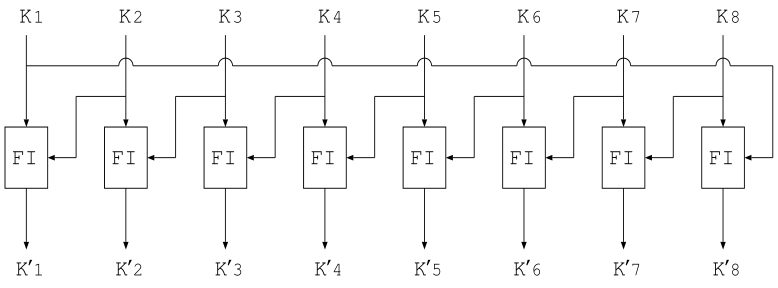
\includegraphics[scale=0.35]{misty_key_schedule}
        \caption{Схема розгортання ключа}
    \end{figure}
    \begin{block}{Характеристика системи}
        \begin{description}
            \item[функція $FI$] 205 рівнянь від 82 змінних;
            \item[функція $FO$] 695 рівнянь від 374 змінних;
            \item[key schedule] 1640 рівнянь від 528 змінних;
            \item[раунд] 1640 рівнянь від 988 змінних;
            \item[шифр] 8448 рівнянь від 3680 змінних.
        \end{description}
    \end{block}
\end{frame}

\begin{frame}[shrink]{Блоковий симетричний шифр MISTY1}{Алгебраїчний криптоаналіз}
    \begin{block}{Апаратне забезпечення}
        \begin{description}
            \item[CPU] Intel Core i5-3570;
            \item[RAM] 8~Gb RAM;
            \item[OS] Ubuntu Linux 12.04;
            \item[Software] Sage v5.9;\\
                CryptoMiniSat v3.0.
        \end{description}
    \end{block}
    \begin{block}{Атака}
        \begin{itemize}
            \item Використано 4 пари відкритого та шифрованого тексту;
            \item Відновлено 176 біт використаного підключа;
            \item Вирішено систему 1640 рівнянь від 988 змінних (2 раунди).
            \item Час обчислення $~50$ год.
        \end{itemize}
    \end{block}
\end{frame}

\begin{frame}[shrink]{Охорона праці та безпека в надзвичайних ситуаціях}
    \begin{columns}
        \begin{column}{0.55\textwidth}
            \begin{itemize}
                \item Проаналізовано умови праці на відповідність нормативним
                    документам з техніки безпеки та санітарії. \\[1em]
                \item Побудовано систему взаємодії <<Людина-Машина-Середовище>> з метою
                    виявлення та оцінки можливих небезпечних та шкідливих виробничих
                    факторів. \\[1em]
                \item Розраховано систему кондиціонування приміщення для
                    забезпечення норм мікроклімату.
            \end{itemize}
        \end{column}%
        \begin{column}{0.5\textwidth}
            \begin{figure}[htbp]
                \centering
                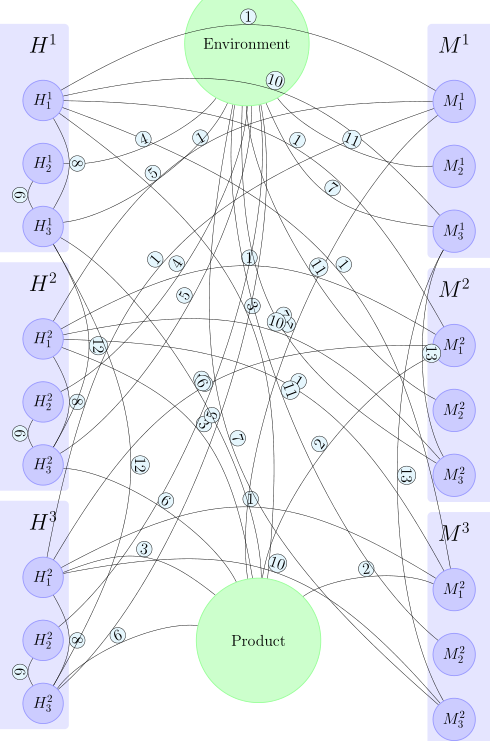
\includegraphics[scale=0.3]{labour_graph}
            \end{figure}
        \end{column}
    \end{columns}
\end{frame}

\begin{frame}{Висновки}
    \begin{itemize}
        \item Запропоновані методи опису рівнянь для криптографічних
            перетворень дозволяють ефективно побудувати систему нелінійних
            рівнянь для більшості сучасних криптоалгоритмів.
        \item Використовуючи описані методики, визначено систему алгебраїчних
            рівнянь для шифрів ГОСТ~28147-89 та MISTY1.
        \item Представлена реалізація досліджуваних криптоалгоритмів
            (ГОСТ~28147-89, MISTY1) дозволяє побудувати відповідні системи
            алгебраїчних рівнянь для аналізу.
            \begin{block}{З використанням представленої реалізації}
                \begin{itemize}
                    \item Вирішено систему рівнянь, що описує 6 раундів шифру ГОСТ~28147-89
                        з відновленням усіх біт використаних підключів.
                    \item Вирішено систему рівнянь, що описує 2 раунди шифру MISTY1
                        з відновленням усіх біт використаних підключів.
                    \item Для більшої кількості раундів можливо знайти еквівалентні ключі.
                \end{itemize}
            \end{block}
        \item Використання ресурсів з потужнішими обчислювальними можливостями
            дозволить підвищити ефективність аналізу.
    \end{itemize}
\end{frame}

\begin{frame}[allowframebreaks]{Список публікацій}
    \scriptsize
    \begingroup
    \renewcommand{\chapter}[2]{}%
    \begin{thebibliography}{1}
            \providecommand*{\BibEmph}[1]{#1}
            \providecommand*{\cyrdash}{\hbox to.8em{--\hss--}}
            \providecommand*{\BibDash}{\ifdim\lastskip>0pt\unskip\nobreak\hskip.2em\fi\cyrdash\hskip.2em\ignorespaces}

            \bibitem{Kiyanchuk:DESSERT:2012}
            \BibEmph{Oliynykov~R.~V., Kiyanchuk~R.~I.} 
            \newblock {Perspective Symmetric Block Cipher optimized for Hardware Implementation}~ 
            \newblock {6-th International Conference ``Dependable Systems, Services \& Technologies (DESSERT'12)''}. \BibDash 2012.

            \bibitem{Kiyanchuk:visnyk:2012}
            \BibEmph{Kiyanchuk~R.~I., Oliynykov~R.~V.} \newblock {Linear transformation properties of
            ZUC cipher}~ \newblock \BibEmph{Visnyk}. \BibDash 2012. \BibDash{Mathematical modeling. Information technologies. Computer-aided
            control systems.}

            \bibitem{karazina:zuc}
            \BibEmph{{Kiyanchuk, R. I. and Oliynykov R. V.}} \newblock {Linear transformation
            properties of ZUC cipher}~ \newblock {Computer modeling in high-end technologies}~/
            Kharkiv national university of radio electronics. \BibDash {Kharkiv}, 2012. \BibDash P.~199 -- 202.

            \bibitem{Kiyanchuk:2012:Banking}
            \BibEmph{Кіянчук~Р.~І.} \newblock {Диференційний аналіз S-функцій}~ 
            \newblock {Наукові дослідження молоді вирішенню проблем європейської інтеграції}~/
            Харківський університет банківської справи. \BibDash Харків, 2012.
            \BibDash Електронне видання на CD-ROM.

            \bibitem{Kiyanchuk:2012:MMF}
            \BibEmph{Кіянчук~Р.~І.} \newblock {Диференційний аналіз S-функцій}~ 
            \newblock {Радіоелектроніка та молодь у XXI столітті}~/ Харківський
            національний університет радіоелектроніки. \BibDash Харків, 2012. \BibDash {с.}~130 -- 131.

            \bibitem{Kiyanchuk:2011:MMF}
            \BibEmph{Кіянчук~Р.~І.} \newblock {Порівняльний аналіз
            IDEA-подібних блочних симетричних шифрів}~ \newblock {
            Міжнародна конференція ``Комп'ютерна інженерія''}~/ 
            Харківський національний університет радіоелектроніки. \BibDash
            Харків, 2011. \BibDash {с.}~225 -- 227.

            \bibitem{Kiyanchuk:IREF:2011:present}
            \BibEmph{Олійников~Р.~В., Кіянчук~Р.~І.} 
            \newblock{Перспективний блоковий симетричний шифр оптимізований для
            апаратної реалізації}~ 
            \newblock{Міжнародна конференція ``Телекомунікаційні системи та
            технології''}~/ 
            Харківський національний університет радіоелектроніки.
            \BibDash Т.~II. \BibDash {Харків, Україна}, 2011. \BibDash 
            с.~321 -- 330.

            \bibitem{Kiyanchuk:2011:Customs}
            \BibEmph{Олейников, Р.~В. and Киянчук, Р.~И.} 
            \newblock{Использование Т-функций в симметричных криптографических преобразованиях}~ 
            \newblock{Материалы международной научно-практической конференции <<Перспективы
            развития информационных и транспортно-таможенных технологий в таможенном
            деле, внешнеэкономической деятельности и управлении организациями>>}~/ 
            {Харьковский национальный университет радиоэлектроники}. \BibDash Днепропетровск, 2011. \BibDash 
            {c.}~213 -- 215.

            \bibitem{Kiyanchuk:2009:rijndael}
            \BibEmph{Долгов, В.~И. and Лисицкая, И.~В. and Киянчук, Р.~И.} 
            \newblock {RIJNDAEL -- это новое или хорошо забытое старое?}~ 
            \newblock{Компьютерные Науки и Технологии}~/ \BibDash
            2009. \BibDash с.~32 -- 35.

            \bibitem{Kiyanchuk:2012:kyiv}
            \BibEmph{Олейников, Р. В.,  Киянчук, Р. И.,  Горбенко, И. Д.}
            \newblock {Алгебраический криптоанализ ГОСТ~28147-89}~ 
            \newblock {XV Юбилейная Международная научно-практическая конференция 22--25 мая 2012}~/ 
            Харьковский национальный университет радиоэлектроники. \BibDash Киев, 2012. \BibDash {с.}~130 -- 131.

            \bibitem{Kiyanchuk:2013:MMF}
            \BibEmph{Киянчук~Р.~І.} \newblock {Алгебраический криптоанализ ГОСТ~28147-89}~ 
            \newblock {Радиоэлектроника и молодёжь в XXI веке}~/ 
            Харьковский национальный университет радиоэлектроники. \BibDash Харків, 2013. \BibDash {с.}~119 -- 120.
    \end{thebibliography}
\endgroup
\end{frame} 

\end{document}
